\documentclass{article}

% \usepackage{savetrees}
\usepackage{fullpage}
\usepackage{apacite}
\usepackage{graphicx}
\usepackage{amsmath}
\usepackage{amsfonts}
\usepackage[titletoc,title]{appendix}
\usepackage{tikz}
\usetikzlibrary{matrix,arrows,decorations.pathmorphing}

\newcommand{\w}[1]{\emph{#1}}
\newcommand{\s}[1]{``#1''}
\newcommand{\myname}[1]{\underline{#1}}

\title{Language meaning at different levels of abstraction}
\author{Erin Bennett}
\date{\today}

% it should recap the work you've done and sketch out the work you are proposing to do to form your thesis
\begin{document}
   \maketitle
   
   \section{Introduction}

   I have two main sections of work that address language meaning.
   In the first section, I discuss several extensions to a pragmatic model of scalar adjectives.
   In the second, I discuss sentence vectors and discourse: how to learn sentence representations from discourse relations, and how to describe discourse dynamics in terms of sentence vectors.

   \section{Adjectives}

   \subsection{Intensifiers}

   In our paper \cite{BennettGoodman2018}, we extend \citeA{Lassiter2013}'s model (Appendix \ref{sec:adj_model}) to cover adjective phrases with intensifying adverbs (e.g. \w{extremely}, \w{very}).
   We assume that each intensified adjective phrase $i$ has its own threshold $\theta_i$ and include the bare adjective, the intensified adjective, and \w{no utterance} as possible alternatives.
   These alternative utterances vary in their cost $c_i$, which the pragmatic listener can use to infer the thresholds.

    % based on \citeA{Lassiter2013}'s model of scalar adjectives.
   In a series of MTurk studies, we demonstrate that, as predicted by this model, longer and less frequent intensified adjective phrases correspond to higher values (Figure \ref{fig:intensifiers}).
   The effect of length holds for even novel intensifiers, inducating that this can be an active, on-line inference.
   % We also show that people use the length of a novel intensifier to actively infer its meaning.
   % The effect of length holds for novel intensifiers, indicating that the length of an intensifier can cause its interpretation to be higher in an on-line inference.

   \begin{figure}[bht]
      \begin{center}
         \includegraphics[width=0.38\textwidth]{images/exp1-q.png}
         \includegraphics[width=0.3\textwidth]{images/height-by-cost.pdf}
         \includegraphics[width=0.3\textwidth]{images/plot_study1b.pdf}
      \end{center}
      \caption{Screenshot, model predictions, and results of Intensifiers study 1b. As surprisal increases, participants' scaled responses increase.} 
      \label{fig:intensifiers}
   \end{figure}

   \subsubsection{Next steps for Intensifiers}

   This section could be complete as is, or could be extended in the following ways:

  	\begin{itemize}
      \item{The pragmatic model currently makes a qualitative prediction.
      But we could specify more details and quantitatively predict responses.
      This would require both a specific way to calculate utterance cost (which the linear regression models in the paper would basically provide) and the prior distributions over prices (which we also need for the sorites section).}
      \item{The model predicts that as intensifiers become more frequent, they will lose their strength.
      We could try to test this prediction, e.g. by manipulating the frequencies of adverbs within an experiment or by somehow estimating the strength of intensifiers from historical corpora.}
   \end{itemize}

   \subsection{Sorites}

   Also based on \citeA{Lassiter2013}'s model of scalar adjectives, we (Dan Lassiter, Noah, and I) explored the ``paradox of the heap'', or \emph{sorites} paradox.
   The observation is that the following two premises seem true:

   \begin{align*}
   \text{A million grains of sand is a heap of sand. }&\text{\emph{(Concrete premise)}} \\
   \text{A heap of sand with one grain of sand taken away is still a heap. }&\text{\emph{(Inductive premise)}}
   \end{align*}

   However, if these premises actually are both completely true, then we should be able apply the inducitive premise thousands of times and conclude that a single grain of sand is a heap.

   We can resolve this paradox with \citeA{Lassiter2013}'s model if the threshold $\theta$ for a scalar adjective is inferred separately in each of its different contexts.
   We use the adjective \w{expensive} and explore the following premises for different values of $V$ and $\varepsilon$.

   \begin{align*}
   \text{A sweater that costs \$$V$ is expensive. }&\text{\emph{(Concrete premise)}} \\
   \text{A sweater that costs \$$\varepsilon$ less than an expensive sweater is expensive. }&\text{\emph{(Inductive premise)}}
   \end{align*}

   We collected ratings for the concrete and inductive premises for the adjective \w{expensive} for different objects and dollar amounts and compared these ratings to model predictions.
   Qualitatively, we show that as the difference amount $\varepsilon$ increases, people are less and less willing to endorse the inductive premise.

   The meaning of \w{expensive} for a sweater depends on the distribution over prices for sweaters.
   We elicited price distributions for five different objects using a binned histogram method \cite{franke2016cogsci}.

   We initially modeled the concrete premise and inductive premises by first using the pragmatic listener's inference of the price $d$ and threshold $\theta$ for \s{The sweater is expensive.}
   For the concrete premise, we then determined whether $V$ was above or below $\theta$.
   For the inductive premise, we determined whether $d-\varepsilon$ was above $\theta$.

   \begin{figure}[bht]
      \begin{center}
         \includegraphics[width=0.5\textwidth]{images/sorites.png}
         \includegraphics[width=0.3\textwidth]{images/sorites-scatter.png}
      \end{center}
      \caption{Best model fit for sorites studies.} 
      \label{fig:sorites}
   \end{figure}

   Using these semantics and a log-normal fit to our binned histogram data, we found a reasonable model fit to human endorsements (Figure \ref{fig:sorites}).
   However, our number of participants was small, model fit is very sensitive to the prior elicitation method, and the semantics we used was pretty clunky.
   We attempted to run a BDA with these semantics on all of our pilot studies together and got a very poor fit ($R^2=0.12$).

   \subsubsection{Next steps for Sorites}

   I'd like to run a replication with the following changes:

   \begin{itemize}
      \item{Choose number of participants with a power analysis.}
      \item{Clean up concrete prompts to set up for an $S_1$ model:
      \begin{align*}
         &\text{Noah bought a sweater for \$V.} \\
         &\text{How much do you agree with the following statement:} \\
         &\text{\bf The sweater was expensive.}
      \end{align*}
      }
      \item{Clean up inductive prompts to set up for an $S_1$ model:
      \begin{align*}
         &\text{Noah bought a sweater. Noah's sweater was expensive.} \\
         &\text{Mike bought a different sweater for \$$\varepsilon$ less.} \\
         &\text{How much do you agree with the following statement:} \\
         &\text{\bf Mike's sweater was expensive.}
      \end{align*}
      }
      \item{Use a pragmatic speaker $S_1$ as an endorsement model for the premises \cite{DegenGoodman2014-Cogsci, franke2014typical}.
      \begin{align*}
         [[\text{The sweater was expensive.}]]^{V, \theta} =& \begin{cases}
             1, & \text{if } V>\theta \\
             0, & \text{otherwise}
         \end{cases} \\
         \text{Concrete Endorsement} =& S_1(\text{\s{The sweater was expensive}}| d=V) \\
         \text{Inductive Endorsement} =& S_1(\text{\s{The sweater was expensive}} | d_{Mike}=(d_{Noah}-\varepsilon)) \\
         & \text{where } d_{Noah} \sim L_1(\text{\s{The sweater was expensive}})
      \end{align*}
      }
      \item{Assume lognormal priors, since this was empirically a good fit, and it lets us get quality estimates for the tails of distributiions.}
      \item{Use BDA for prior and endorsement data jointly}
   \end{itemize}


   %  semantics isn't 

   % In the concrete premise, the threshold for the adjective \w{expensive} depends only on the prior distribution over prices of sweaters.
   % In our first version of this project, we simply evaluate the truth of the concrete premise by checking whether $V$ is greater than or equal to the inferred threshold for a sentence like \s{This sweater is expensive.}.
   % We will reimplement model predictions using a pragmatic speaker for the endorsement model \cite{DegenGoodman2014-Cogsci, franke2014typical}.


   % In the inductive premise, the 

   
   % 

   \section{Sentence vectors}

   \subsection{DisSent}

   In our manuscript \cite{NieBennettGoodman17}, we use marked discourse relations (e.g. \w{but}, \w{because}, \w{so}) to learn sentence vectors.
   This is a self-supervised method, where we extract pairs of sentences using dependency parsing (Figure \ref{fig:dissent}).
   We then use a model developed for supervised sentence relation pairs \cite{conneau2017supervised} to jointly train the individual sentence vectors and a classifier that uses those vectors to predict the relation.
   On a variety of generalization tasks that depend on sentence meaning, we use sentence vectors as features for a simple logistic regression.
   DisSent vectors perform well relative to state-of-the-art sentence vectors (Figure \ref{fig:dissent}).

   % This section could be complete as is, or it could be extended in the following ways:
   % \begin{itemize}
   %    \item{???}
   %    \item{multilingual}
   % \end{itemize}

   \begin{figure}[bht]
    \centering
    \footnotesize
    % \begin{subfigure}{0.5\textwidth}
        \begin{tikzpicture}
            \node (S1)[shape=rectangle,draw=black,rounded corners]
                at (0, 2.5) {S1};
            \node (because)[shape=rectangle,draw=black,rounded corners]
                at (2, 2.5) {because};
            \node (S2)[shape=rectangle,draw=black,rounded corners]
                at (4, 2.5) {S2};
            \node (sentence)
                at (2, 2) {It hated me because I talked to it.};

            \path [->] (S1) edge[bend left=60]
                node[above] {advcl} (S2);
            \path [->] (S2) edge[bend right=30]
                node[above] {mark} (because); 
    %     \end{tikzpicture}
    %     \caption{one version}
    %     \label{S1becauseS2}
    % \end{subfigure}
    % \begin{subfigure}{0.5\textwidth}
    %     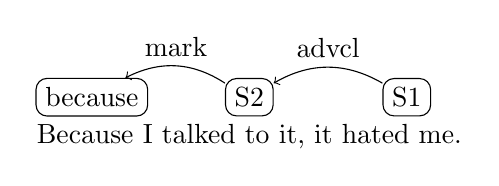
\begin{tikzpicture}
            \node (S1)[shape=rectangle,draw=black,rounded corners]
                at (4, 0.5) {S1};
            \node (because)[shape=rectangle,draw=black,rounded corners]
                at (0, 0.5) {because};
            \node (S2)[shape=rectangle,draw=black,rounded corners]
                at (2, 0.5) {S2};
            \node (sentence)
                at (2, 0) {Because I talked to it, it hated me.};

            \path [->] (S1) edge[bend right=30]
                node[above] {advcl} (S2);
            \path [->] (S2) edge[bend right=30]
                node[above] {mark} (because); 
         \end{tikzpicture}
         \hspace{0.5cm}
         \includegraphics[width=0.55\textwidth]{images/dissent.png}

    %     \caption{another version}
    %     \label{becauseS2S1}
    % \end{subfigure}
    \caption{Dependency relations used for extraction and generalization performance of DisSent sentence vectors relative to Skipthought and InferSent.}
    \label{fig:dissent}
\end{figure}

   \subsubsection{Next steps for DisSent}

   % These sentence vectors are useful, but they obviously don't capture sentence meaning perfectly.
   This section could be complete as is, but it would be cool if we could make better sentence vectors.
   These sentence vectors are useful, but they obviously don't capture sentence meaning perfectly.

   One possible direction to improve embeddings would be to use other kinds of self-supervision (e.g. punctuation).

   Another direction is to develop a model of discourse markers that better captures how people use them in natural language.
   With a model that more accurately captures how people use discourse markers, we might be able to use them more effectively to learn sentence vectors.
   % Possibly if we developed a model based on a deeper understanding of discourse relations and the flow of a discourse.
   We've spent some time brainstorming models where different discourse markers are modeled as transoformations, e.g. a function from the meaning of S1 to the meaning of S2, or from the previous topic of the discourse to a new topic.
   It's possible that the next section, in which we describe the trajectories of documents within a given sentence embedding space, could inspire more interesting models for training better sentence vectors.
    % from the previous sentence's representation to the next sentence's representation.
   % from the discourse vector used to generate S1 to the discourse vector used to generate S2.
   % one sentence representation to another.

   \subsection{Describing discourse dynamics}

   Given a way of computing sentence vectors, how can we describe the trajectories of different kinds of documents through this high-dimensional space?

   % My plan is to present visualizations and statistics on the dynamics of discourse across a range of corpora. We can look at differences between genres, markers of coherence (discourse markers, paragraph boundaries, etc.), and qualitative differences between sensible and nonsensical, impossible, or unusual sentence vectors.

   I've collected some visualizations for Skipthought vectors of Wikipedia sentences.
   We see greater similarity between nearby sentences than further away sentences in a document, indicating a kind of graded coherence.
   This coherence exists within paragraph boundaries but across paragraph boundaries we tend to get especially high displacements (Figure \ref{fig:dnd}).
   % My plan is to look at how these dynamics vary across different genres. We will find out whether different explicit markers of discourse relations and coherence (transition words like “because”, different kinds of punctuation, etc.) signal systematic displacements in the meaning of the two surrounding sentences. We will show where in discourse space typical sentence meanings fall in contrast to where nonsensical or unusual sentence meanings, describing a “prior over sentence meanings”.

   \begin{figure}[bht]
      \begin{center}
         \includegraphics[width=0.45\textwidth]{images/decay.png}
         \includegraphics[width=0.5\textwidth]{images/within-vs-across-paragraphs.png}
      \end{center}
      \caption{The distance between a random sentence in a document and the sentence N steps away increases exponentially in general. But the distances between sentences separated by only a paragraph boundary are even higher than between two random, distant sentences in a document.} 
      \label{fig:dnd}
   \end{figure}

   \subsubsection{Next steps for Discourse Dynamics}

   This is the most open-ended project.
   Some of the questions I'd like to address are:
   \begin{itemize}
      \item{What kinds of displacements occur across paragraphs, different kinds of punctuation, different discourse markers, etc..
      Can we predict the relation from the displacement?
      Do some seperators have higher or lower displacement magnitudes?}
      \item{What do different genres, modalities, writers, speakers, etc. share in their discourse dynamics? How do they differ?}
      \item{Can we differentiate the kinds of sentence vectors that will correspond to sensible meanings vs. unusual, nonsensical, or impossible meanings?}
      \item{Do different sentence embedding models lead to different descriptions of discourse dynamics? How so?}
      \item{How might the descriptions of the resulting discourse spaces and trajectories inform sentence embedding models?}
   \end{itemize}

   \bibliographystyle{apacite}
   \bibliography{first_committee_meeting}

   \begin{appendices}

      \section{Adjective model \label{sec:adj_model}}

   The intensifiers and sorites sections are based on \citeA{Lassiter2013}'s RSA model of scalar adjectives.
   % In this model, for the sentence \s{X is expensive}, a listener considers two possible utterances: the one that was actually said, or nothing.
   In this model, the meaning of the adjective depends on a threshold parameter $\theta$.
   For the adjctive \w{expensive}, the adjective is true of an object X when the price of X is greater than $\theta$.

   \begin{align*}
      % u &\in \left\{ \text{\s{X is expensive}, \w{no utterance}} \right\} \\
      d &= price(X) \\
      [[\text{\w{no utterance}}]](d, \theta) &= 1 \\
      [[\text{X is expensive}]](d, \theta) &= \begin{cases}
          1, & \text{if } d>\theta \\
          0, & \text{otherwise}
      \end{cases} \\
   \end{align*}


   The price and threshold are jointly inferred by a pragmatic listener according to RSA \cite{GoodmanFrank2016-TICS}.


   \begin{align*}
      L_0(d|u, \theta) &\propto \delta_{[[u]](d, \theta)} \cdot P(d) \\
      S(u | d, \theta) &\propto e^{
         \alpha \left( \log[L_0(d|u, \theta)] - c \right)
      } \\
      L_1(d, \theta | u) &\propto S(u|w, \theta) \cdot P(w) \cdot P(\theta)
   \end{align*}

   % I've worked on two projects extending \citeA{Lassiter2013}'s RSA model of scalar adjectives.
   % In this model, for the sentence \s{X is expensive}, a listener considers two possible utterances: the one that was actually said, or nothing.

   % \begin{align*}
   %    & u \in \left\{ \text{\s{X is expensive}, \w{no utterance}} \right\}
   % \end{align*}

   % The pragmatic listener $L_1$ jointly infers a dollar amount $d$ for the price of X and a threshold parameter $\theta$ for the scalar adjective \w{expensive}.
   % This inference is based on the prior probability of each price $P(d)$ and parameter $P(\theta)$ and the likelihood -- the probability that a speaker would choose that utterance.

   % \begin{align*}
   %    d &= price(X) \\
   %    L_1(d, \theta | u) &\propto S(u|w, \theta) \cdot P(w) \cdot P(\theta)
   % \end{align*}

   % The speaker $S$ chooses an utterance $u$ by soft-maximizing (with parameter $\alpha$) informativity $log(L_0(d|u, \theta))$ minus cost $c$.

   % \begin{align*}
   %    &S(u | d, \theta) \propto e^{
   %       \alpha \left( \log[L_0(d|u, \theta)] - c \right)
   %    }
   % \end{align*}

   % Informativity is based on the literal listener $L_0$, which conditions on the meaning of the utterance $[[u]]$ and reweights based on the prior probability of the world $w$.

   % \begin{align*}
   %    L_0(d|u, \theta) &\propto \delta{[[u]]^{d, \theta}} \cdot P(d) \\
   % \end{align*}

   % The literal meaning of the adjective \w{expensive} is whether the price $d$ is above the parameter $\theta$, and the literal meaning for saying nothing is trivially true.

   % \begin{align*}
   %    [[\text{\w{no utterance}}]]^{d, \theta} &= 1 \\
   %    [[\text{X is expensive}]]^{d, \theta} &= \begin{cases}
   %        1, & \text{if } d>\theta \\
   %        0, & \text{otherwise}
   %    \end{cases}
   % \end{align*}


   %  the literal listener infers a price $d$ given an utterance $u$ and some parameters $\theta$ based on the truth value of the utterance for that price $[[u]]^{d, \theta}$ and the prior probability of that price $P(d)$.
   % Given a known price $d$, the speaker $S$ soft-maximizes (with parameter $\alpha$) informativity $log(L_0(d|u, \theta))$ minus cost cost $c$ to choose an utterance $u$.
   % Finally, the pragmatic listener infers both the price and parameters 

   % In this model, the literal listener $L_0$ hears an utterance $u$ and uses some parameters $\theta$ and lexicon $\mathcal{L}$ to infer a state of the world $w$.
   % The probability of the literal listener returning each world state depends on its prior probability $P(w)$ and the meaning of the utterance $[[u]]$ in that world and under that lexicon.
   % The speaker knows the world $w$ and uses a softmax (with parameter $\alpha$) on the informativity $L_0$ and cost $c$ of each utterance $u$ to decide what to say.
   % The pragmatic listener $L_1$ infers both the world $w$ and parameters $\theta$ given the utterance according to the prior probabilities of the parameters $P(\theta)$ and of the world $P(w)$ and the likelihood of the speaker choosing the utterance $u$ in that world.


      \section{Other open questions}

      \paragraph{Multilingual DisSent} We worked on generalizing our results for English to other languages, but got poor results, likely due to the inferier quality of the word embeddings and a need to tune the extraction method to these other languages.

      \paragraph{Intensifiers and negation}

      Intensifiers behave in interesting ways with negation (\w{not very tall}).
      % That is, we either mean that there's a threshold for \w{happy} that this person falls below (\w{not [unhappy]}), or we mean that there's a threshold for \w{unhappy} which this person falls above.
      % Based on their ranges (e.g. existence of min/max values) different adjectival scales behave differently with \w{not very} 
      \citeA{leffel2016vagueness} showed that different adjective scales behave differently with \w{not very} (e.g. \w{not very late} necessarily means late, whereas \w{not very fast} doesn't necessarily mean fast).
      \citeA{tesslernot} extended our intensifiers model to account for double-negated scalar adjectives (e.g. \w{not unhappy}) that essentially included ambiguity over the negation scope, and this could be a nice starting point to modeling negated intensifiers.

      \paragraph{Alternative or lesioned models for sorites}

      It might be nice to have alternative models to compare to.

      % \section{Other past projects and collaborations}
      % In order of completeness:

      % \paragraph{Eliciting prior distributions} I helped with this CogSci paper exploring different dependent measures for eliciting prior expectations about quantities like prices, heights, and likely outcomes \cite{franke2016cogsci}.

      % \paragraph{Mindsets} We wrote up a PPL model of growth vs. fixed mindsets. We identified different variables in the model (goals, theory of how effort influences immediate success vs. long-term abilities, etc.) and ran an MTurk experiment to see whether any of those variables corresponded to mindset scale scores. Our elicitation questions didn't get a lot of variation in responses, and our findings were inconclusive.

      % \paragraph{Scripts} [fyp writeup]
      % \paragraph{Counterfactual explanations} [end of internships writeup]
      % \paragraph{ROCstories} [class writeup]
      % \paragraph{Whybot} [presentations and experiments]
      % \paragraph{MetaRL} [class proposal]
      % \paragraph{CFGANS} [some experiments documented, and sahil's class writeup]
      % \paragraph{Adjective morphs} [experiments and model results]
      % \paragraph{Text adventure} [a little demo]

   \end{appendices}

\end{document}
